\documentclass[10pt,a4paper]{ltjsarticle}       % LuaTeX を使う
    \usepackage[luatex]{graphicx}             % LuaTeX 用, draft がついているときは図の代わりに同じ大きさの枠ができる
    \usepackage{here}                               % 図表の位置を強制して出力
    \usepackage{afterpage}                          % 残っている図を貼り付ける(\afterpage{\clearpage})
    \usepackage[subrefformat=parens]{subcaption}    % サブキャプション(図1(a) とか)
    \usepackage{setspace}                           % 行間制御
    \usepackage{ulem}                               % 下線や取り消し線など
    \usepackage{booktabs}                           % きれいな表(\toprule \midrule \bottomrule)
    \usepackage{multirow}                           % 表で行結合
    \usepackage{multicol}                           % 表で列結合
    \usepackage{hhline}                             % 表で 2 重線
    \usepackage[table]{xcolor}                      % カラー
    \usepackage{tikz}                               % 図描画用
    \usepackage[framemethod=tikz]{mdframed}         % 文章を囲むとき用
    \usepackage[version=3]{mhchem}                  % 化学式
    \usepackage{siunitx}                            % 単位
    \usepackage{comment}                            % コメント
    \setcounter{tocdepth}{3}                        % 目次に subsubsection まで表示
    \usepackage{listings}
    \lstset{
        frame=single,
        basicstyle=\small\ttfamily,
        tabsize=4,
        language=python,
        keywordstyle=\color{red},
        stringstyle=\color{blue}
    }

    % -----ヘッダ・フッタの設定-----
    \usepackage{fancyhdr}
    \usepackage{lastpage}
    \pagestyle{fancy}
    \lhead{}                                 % 左ヘッダ
    \chead{}                                 % 中央ヘッダ
    \rhead{}                                 % 右ヘッダ
    \lfoot{}                                 % 左フッタ
    \cfoot{\thepage~/~\pageref{LastPage}}    % 中央フッタ
    \rfoot{}                                 % 右フッタ
    \renewcommand{\headrulewidth}{0pt}       % ヘッダの罫線を消す
    % -----余白の設定-----
    % これをアンコメントするとページ番号が中央からずれるから今は使わない.
    % \usepackage[left=19.05mm,right=19.05mm,top=25.40mm,bottom=25.40mm]{geometry}
    % -----フォントの設定-----
    % https://ja.osdn.net/projects/luatex-ja/wiki/LuaTeX-ja%E3%81%AE%E4%BD%BF%E3%81%84%E6%96%B9
    % http://myfuturesightforpast.blogspot.jp/2013/12/tex-gyre.html など
    \usepackage[no-math]{fontspec}
    \usepackage{amsmath,amssymb}    % 高度な数式用
    \usepackage{mathrsfs}           % 花文字用
    % times ベース -> txfonts
    % palatino ベース -> pxfonts
    \usepackage{txfonts}
    \usepackage{bm}                 % 斜体太字ベクトル
    % Avant Garde -> TeX Gyre Adventor
    % Bookman Old Style -> TeX Gyre Bonum
    % Zapf Chancery -> TeX Gyre Chorus
    % Courier -> TeX Gyre Cursor
    % Helvetica -> TeX Gyre Heros
    % Helvetica Narrow -> TeX Gyre Heros Cn
    % Palatino -> TeX Gyre Pagella
    % New Century Schoolbook -> TeX Gyre Schola
    % Times -> TeX Gyre Termes
    \setmainfont[Ligatures=TeX]{TeXGyreTermes}
    \setsansfont[Ligatures=TeX]{TeXGyreHeros}
    \setmonofont[Scale=MatchLowercase]{TeXGyreCursor}
    \usepackage[match,deluxe,expert,bold]{luatexja-fontspec}
    \setmainjfont[BoldFont=IPAexGothic]{IPAexMincho}
    \setsansjfont{IPAexGothic}
    \usepackage{luatexja-otf}
    % -----PDF ハイパーリンク,ブックマーク,URL の設定-----
    % オプション(\hypersetup{})は https://texwiki.texjp.org/?hyperref 参照
    \usepackage{url}
    % -----ソースコードの設定-----
    % オプション(\lstset{})は http://tug.ctan.org/tex-archive/macros/latex/contrib/listings/listings.pdf 参照
    % 使うときは
    % \begin{lstlisting}[language=aaaa,caption=bbbb,label=List:cccc]
    % hogehoge
    % \end{lstlisting}
    \usepackage{listings}
    \lstset{%
      basicstyle=\ttfamily\small,%
      frame=single,%
      frameround=ffff,%
      numbers=left,%
      stepnumber=1,%
      numbersep=1\zw,%
      breaklines=true,%
      tabsize=4,%
      captionpos=t,%
      commentstyle=\itshape}
    % -----図表等の reference の設定-----
    % 表示文字列を日本語化
    \renewcommand{\figurename}{図}
    \renewcommand{\tablename}{表}
    \renewcommand{\lstlistingname}{リスト}
    \renewcommand{\abstractname}{概要}
    % 図番号等を"<章番号>.<図番号>"
    % lstlisting に関しては https://tex.stackexchange.com/questions/134418/numbering-of-listings 参照
    \renewcommand{\thefigure}{\thesection.\arabic{figure}}
    \renewcommand{\thetable}{\thesection.\arabic{table}}
    \AtBeginDocument{\renewcommand{\thelstlisting}{\thesection.\arabic{lstlisting}}}
    \renewcommand{\theequation}{\thesection.\arabic{equation}}
    % 節が進むごとに図番号等をリセット
    % http://d.hatena.ne.jp/gp98/20090919/1253367749 参照
    \makeatletter
    \@addtoreset{figure}{section}
    \@addtoreset{table}{section}
    \@addtoreset{lstlisting}{section}
    \@addtoreset{equation}{section}
    \makeatother
    % \ref{} の簡単化
    \newcommand*{\refSec}[1]{\ref{#1}~章}
    \newcommand*{\refSsec}[1]{\ref{#1}~節}
    \newcommand*{\refSssec}[1]{\ref{#1}~項}
    \newcommand*{\refFig}[1]{\figurename~\ref{#1}}
    \newcommand*{\refTab}[1]{\tablename~\ref{#1}}
    \newcommand*{\refList}[1]{\lstlistingname~\ref{#1}}
    \newcommand*{\refEq}[1]{式~(\ref{#1})}
    % -----数式中便利な定義-----
    % https://www.library.osaka-u.ac.jp/doc/TA_LaTeX2.pdf
    % https://en.wikibooks.org/wiki/LaTeX/Mathematics など
    \newcommand{\e}{\mathrm{e}}                     % ネイピア数
    \newcommand{\imagi}{\mathrm{i}}                 % 虚数単位(i)
    \newcommand{\imagj}{\mathrm{j}}                 % 虚数単位(j)
    \newcommand{\vDel}{\varDelta}                   % デルタ大文字
    \newcommand{\veps}{\varepsilon}                 % イプシロン小文字
    \newcommand*{\paren}[1]{\left( #1 \right)}      % () を中身の大きさに合わせる
    \newcommand*{\curly}[1]{\left\{ #1 \right\}}    % {} を中身の大きさに合わせる
    \newcommand*{\bracket}[1]{\left[ #1 \right]}    % [] を中身の大きさに合わせる
    \renewcommand{\Re}{\operatorname{Re}}           % 実部
    \renewcommand{\Im}{\operatorname{Im}}           % 虚部
    \newcommand*\sfrac[2]{{}^{#1}\!/_{#2}}          % xfrac パッケージの \sfrac{}{} の代わり
    \renewcommand*\vec[1]{\mathbf{#1}}              % 矢印ベクトルは使わないので上書き.太字立体.
    \newcommand{\argmax}{\mathop{\rm arg~max}\limits}
    \newcommand{\argmin}{\mathop{\rm arg~min}\limits}

    \title{知能システム論第5回課題}
    \author{37186305\\航空宇宙工学専攻修士一年\\荒居秀尚}
    
    \begin{document}
    \maketitle
    \section{宿題1}
    $f(\bm{x}) = \frac{1}{2}\bm{x}^{T}\bm{A}\bm{x}$のとき、$\alpha=1/2$のアルミホ規準は
    \begin{align}
      g(\epsilon_k) &= \frac{1}{2} (\bm{x} - \epsilon_k \bm{A}\bm{x})^{T} \bm{A} (\bm{x} - \epsilon_k \bm{A} \bm{x}) - \frac{1}{2} \bm{x}^{T} \bm{A} \bm{x} \\
                          &= \frac{1}{2} \bm{x}^{T} (\bm{I} - \epsilon_k \bm{A})^{T} \bm{A} (\bm{I} - \epsilon_k \bm{A}) \bm{x} -  \frac{1}{2} \bm{x}^{T} \bm{A} \bm{x} \\
                          &= -\frac{1}{2} \epsilon_k \bm{x}^{T} \bm{A}^{T} \bm{A} \bm{x} - \frac{1}{2} \epsilon_k (\bm{x}^{T} \bm{A}^2 \bm{x} - \epsilon_k \bm{x}^T \bm{A}^T \bm{A}^2 \bm{x}) \\
                          &\le \alpha \epsilon_k g^{\prime} (0) = -\frac{1}{2} \epsilon_k \bm{x}^{T} \bm{A}^{T} \bm{A} \bm{x}
    \end{align}
    これを満たす最大の$\epsilon_k$は等号が成り立つときに得られるため、$\bm{A}$が正定値対称行列であるとすれば、
    \begin{equation}
    \epsilon_k = \frac{\bm{x}^T\bm{A}^2\bm{x}}{\bm{x}^T\bm{A}^3\bm{x}}
    \end{equation}
    
    \section{宿題2}
    $f(\bm{x}) = \frac{1}{2}\bm{x}^T\bm{A}\bm{x}$に対する厳密直線探索を用いた最急降下法において
    \begin{align}
    \bm{x}_{k+1} &= \bm{x} - \epsilon_k\nabla f(\bm{x}_k) \\
    \nabla f(\bm{x}) &= \bm{A}\bm{x} \\
    \epsilon_{k} &= \frac{\|\nabla f(\bm{x}_k)\|^2}{\nabla f(\bm{x}_k)^T\bm{A}\nabla f(\bm{x}_k)}
    \end{align}
    となる。簡単のため$\nabla f(\bm{x}_k) = \bm{g_k}$と表記すると
    \begin{align}
    f(\bm{x}_{k+1}) &= \frac{1}{2} \left( 
        \bm{x}_k - \frac{
                                   {\bm{g}_k}^T {\bm{g}_k}
                                }{ 
                                   {\bm{g}_k}^T \bm{A}  \bm{g}_k 
                                } \bm{g}_k 
       \right)^T \bm{A}  \left( 
       \bm{x}_k - \frac{
                                 {\bm{g}_k}^T {\bm{g}_k}
                               }{ 
                                 {\bm{g}_k}^T \bm{A}  \bm{g}_k 
                               } \bm{g}_k \right) \\
    &= \frac{1}{2} \bm{x}_k \bm{A} \bm{x}_k - \frac{
                                                                             2 \left({\bm{g}_k}^T \bm{g}_k\right) \left( {\bm{g}_k}^T \bm{A}\bm{x}_k \right) - \left( {\bm{g}_k}^T \bm{g}_k \right)^2 }{ 2{\bm{g}_k}^T \bm{A}\bm{g}_k }
    \end{align}
    ここで、$\bm{g}_k = \bm{A}\bm{x}_k$であることから、上式の第二項は
    \begin{equation}
    \frac{
      2\left( {\bm{g}_k}^T \bm{g}_k \right) \left( {\bm{g}_k}^T \bm{A}\bm{x}_k \right) - \left( {\bm{g}_k}^T \bm{g}_k \right)^2
    }{
      2{\bm{g}_k}^T \bm{A}\bm{g}_k
    } = \frac{
      2\left( {\bm{g}_k}^T \bm{g}_k \right)^2 - \left( {\bm{g}_k}^T \bm{g}_k \right)^2
    }{
      2{\bm{g}_k}^T \bm{A}\bm{g}_k
    } = \frac{
      \left( {\bm{g}_k}^T \bm{g}_k \right)^2
    }{
      2{\bm{g}_k}^T \bm{A}\bm{g}_k
    }
    \end{equation}
    したがって
    \begin{align}
      f(\bm{x}_{k+1}) &= \left( 1 - \frac{
        \left( {\bm{g}_k}^T \bm{g}_k \right)^2
      }{
        \left( {\bm{x}_k}^T \bm{A}\bm{x}_k  \right) \left( {\bm{g}_k}^T \bm{A}\bm{g}_k \right)
      } \right)f(\bm{x}_k) \\
      &= \left( 1 - \frac{
        \left( {\bm{g}_k}^T \bm{g}_k \right)^2
      }{
        \left( {\bm{g}_k}^T \bm{A}^{-1}\bm{g}_k  \right) \left( {\bm{g}_k}^T \bm{A}\bm{g}_k \right)
      } \right)f(\bm{x}_k)
    \end{align}
    カントロビッチの不等式において$c = \frac{1 - \lambda_{min} / \lambda_{max}}{1 + \lambda_{min} / \lambda_{max}}$とおくと
    \begin{equation}
      \frac{
        4\lambda_{min}\lambda_{max}
      }{
        \left( \lambda_{max} + \lambda_{min} \right)^2
      } = 1 - c^2 \le \frac{
        \|\bm{g}_k \|^4
      }{
        {\bm{g}_k}^T \bm{A}^{-1} \bm{g}_k \cdot {\bm{g}_k}^T \bm{A} \bm{g}_k
      }
    \end{equation}
    これにより
    \begin{equation}
    f(\bm{x}_{k+1}) \le c^2 f(\bm{x}_k)
    \end{equation}
    が成り立つ。
    \section{宿題3}
    Julia 1.0.0を用いて実装した。
    \begin{lstlisting}
using Plots

# Functions
f(x, y) = 10x^2 + y^2
df(x) = [20x[1], 2x[2]]

function backtrack(x, epsilon, alpha, beta)
    x_new = x - epsilon .* df(x)
    while f(x_new[1], x_new[2]) - f(x[1], x[2]) > -alpha * epsilon * sum(df(x).^2)
        epsilon *= beta
        x_new = x - epsilon .* df(x)
    end
    x_new
end

# Variables
x = y = range(-5, stop=5, length=100)
p = plot(x, y, f, st = [:contourf])

niter = 5
pos = 10 * rand(2) .- 5
epsilon = 1.0
alpha = 0.5
beta = 0.8
previous = [0.0, 0.0]
for i in 1:niter
    previous = copy(pos)
    pos = backtrack(pos, epsilon, alpha, beta)
    plot!(p[1], [previous[1], pos[1]], [previous[2], pos[2]], line = (:white, 1))
end
    \end{lstlisting}
    結果は以下の図\ref{fig:optim}のようになった。
    \begin{figure}[htbp]
      \begin{center}
        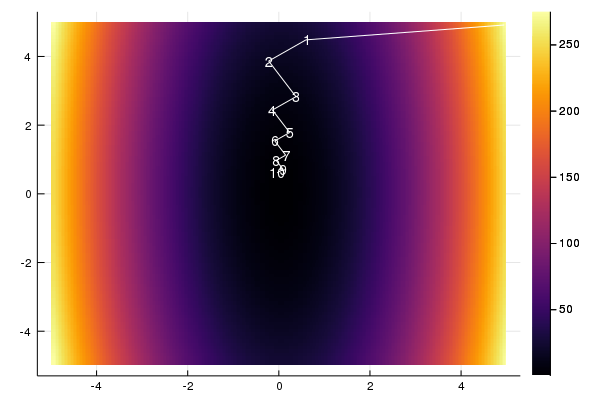
\includegraphics[clip, scale=0.7]{optim.png}
        \caption{バックトラック直線探索を用いた最急降下法}
        \label{fig:optim}
      \end{center}
    \end{figure}
    \section{宿題4}
    \subsection{A}
    BFGSアルゴリズムのヘッセ行列の更新式において
    \begin{align}
    \bm{H}_{k+1} &= \bm{H}_k + \frac{\bm{t}_k {\bm{t}_k}^T}{{\bm{s}_k}^T \bm{t}_k} - \frac{\bm{H}_k\bm{s}_k {\bm{s}_k}^T\bm{H}_k}{{\bm{s}_k}^T\bm{H}_k\bm{s}_k} \\
    &= \bm{B} - \frac{\bm{H}_k\bm{s}_k {\bm{s}_k}^T\bm{H}_k}{{\bm{s}_k}^T\bm{H}_k\bm{s}_k}
    \end{align}
    のように第1項と第2項をまとめて$\bm{B}$と呼ぶことにする。また、スカラー量${\bm{s}_k}^T \bm{t}_k$を$a$と表記することにする。まず、$\bm{B}$ の逆行列についてシャーマン・モリソン公式を用いると
    \begin{equation}
    \bm{B} = \bm{H}_k + \frac{\bm{t}_k {\bm{t}_k}^T} {a}
    \end{equation}
    なので
    \begin{equation}
    \bm{B}^{-1} = {\bm{H}_k}^{-1} - \frac{
      {\bm{H}_k}^{-1}\bm{t}_k{\bm{t}_k}^T{\bm{H}_k}^{-1}
    }{
      a + {\bm{t}_k}^T{\bm{H}_k}^{-1}\bm{t}_k
    }
    \end{equation}
    これを用いて
    \begin{align}
    {\bm{H}_{k+1}}^{-1} &= {\bm{B}}^{-1} + \frac{
      \bm{B}^{-1}\bm{H}_k \bm{s}_k{\bm{s}_k}^T{\bm{H}_k}^T\bm{B}^{-1}
    }{
      {\bm{s}_k}^T\bm{H}_k\bm{s}_k - {\bm{s}_k}^T{\bm{H}_k}^T\bm{B}^{-1}\bm{H}_k\bm{s}_k
    } \\
    &= \bm{B}^{-1} + \frac{
      \bm{B}^{-1}\bm{H}_k \bm{s}_k{\bm{s}_k}^T{\bm{H}_k}^T\bm{B}^{-1}
    }{
      {\bm{s}_k}^T\bm{H}_k\bm{s}_k - {\bm{s}_k}^T{\bm{H}_k}^T\left(  {\bm{H}_k}^{-1} - \frac{
      {\bm{H}_k}^{-1}\bm{t}_k{\bm{t}_k}^T{\bm{H}_k}^{-1}
    }{
      a + {\bm{t}_k}^T{\bm{H}_k}^{-1}\bm{t}_k
    } \right)\bm{H}_k\bm{s}_k
    } \\
    &= \bm{B}^{-1} + \frac{
      \bm{B}^{-1}\bm{H}_k \bm{s}_k{\bm{s}_k}^T{\bm{H}_k}^T\bm{B}^{-1}
    }{
      {\bm{s}_k}^T\bm{H}_k\bm{s}_k - {\bm{s}_k}^T{\bm{H}_k}\bm{s}_k + \frac{
      a^2
    }{
      a + {\bm{t}_k}^T{\bm{H}_k}^{-1}\bm{t}_k
    } 
    } \\
    &= \bm{B}^{-1} + \frac{
      \left( a + {\bm{t}_k}^T{\bm{H}_k}^{-1}\bm{t}_k \right) \left( {\bm{H}_k}^{-1} - \frac{
      {\bm{H}_k}^{-1}\bm{t}_k{\bm{t}_k}^T{\bm{H}_k}^{-1}
    }{
      a + {\bm{t}_k}^T{\bm{H}_k}^{-1}\bm{t}_k
    }\right)\bm{H}_k\bm{s}_k{\bm{s}_k}^T{\bm{H}_k}^T \left( {\bm{H}_k}^{-1} - \frac{
      {\bm{H}_k}^{-1}\bm{t}_k{\bm{t}_k}^T{\bm{H}_k}^{-1}
    }{
      a + {\bm{t}_k}^T{\bm{H}_k}^{-1}\bm{t}_k
    } \right)
    }{
      a^2
    } \\
    &= \bm{B}^{-1} + \frac{
      \left( a + {\bm{t}_k}^T{\bm{H}_k}^{-1}\bm{t}_k \right) \bm{s}_k{\bm{s}_k}^T - \left(  {\bm{H}_k}^{-1}\bm{t}_k{\bm{t}_k}^{T}\bm{s}_k{\bm{s}_k}^{T} + \bm{s}_k{\bm{s}_k}^T\bm{t}_k{\bm{t}_k}^T{\bm{H}_k}^{-1} \right)
    }{
      a^2
    } + \frac{
      {\bm{H}_k}^{-1}\bm{t}_k{\bm{t}_k}^T \bm{s}_k{\bm{s}_k}^T \bm{t}_k{\bm{t}_k}^T{\bm{H}_k}^{-1}
    }{
      a^2\left( a + {\bm{t}_k}^T{\bm{H}_k}^{-1}\bm{t}_k \right)
    }
    \end{align}
    ${\bm{t}_k}^T\bm{s}_k = {\bm{s}_k}^T\bm{t}_k = a$なので
    \begin{align}
    {\bm{H}_{k+1}}^{-1} &= \bm{B}^{-1} + \frac{
      \left( a + {\bm{t}_k}^T{\bm{H}_k}^{-1}\bm{t}_k \right) \bm{s}_k{\bm{s}_k}^T - a\left(  {\bm{H}_k}^{-1}\bm{t}_k{\bm{s}_k}^{T} + \bm{s}_k{\bm{t}_k}^T{\bm{H}_k}^{-1} \right)
    }{
      a^2
    } + \frac{
      a^2{\bm{H}_k}^{-1}\bm{t}_k{\bm{t}_k}^T{\bm{H}_k}^{-1}
    }{
      a^2\left( a + {\bm{t}_k}^T{\bm{H}_k}^{-1}\bm{t}_k \right)
    } \\
    &= {\bm{H}_k}^{-1} + \frac{
      \left( {\bm{s}_k}^T\bm{t}_k + {\bm{t}_k}^T{\bm{H}_k}^{-1}\bm{t}_k \right)\bm{s}_k{\bm{s}_k}^T
    }{
      \left( {\bm{s}_k}^T\bm{t}_k \right)^2
    } - \frac{
      {\bm{H}_k}^{-1}\bm{t}_k{\bm{s}_k}^{T} + \bm{s}_k{\bm{t}_k}^T{\bm{H}_k}^{-1}
    }{
      {\bm{s}_k}^T\bm{t}_k
    }
    \end{align}
    となる。
    \subsection{B}
    $\bm{H}_k$が正定値かつ${\bm{s}_k}^T\bm{t}_k >0$のとき$\bm{H}_{k+1}$が正定値であることを、${\bm{H}_{k+1}}^{-1}$の正定値性から示す。
    \begin{equation}
    {\bm{H}_{k+1}}^{-1} = \left( \bm{I} - \frac{\bm{s}_k{\bm{t}_k}^T}{{\bm{s}_k}^T\bm{t}_k} \right) {\bm{H}_k}^{-1} \left( \bm{I} - \frac{\bm{t}_k{\bm{s}_k}^T}{{\bm{s}_k}^T\bm{t}_k} \right) + \frac{\bm{s}_k{\bm{s}_k}^T}{{\bm{s}_k}^T\bm{t}_k}
    \end{equation}
    と表現できることを用いると零ベクトル出ない任意のベクトル$\bm{z}$を用いた二次形式
    \begin{align}
    \bm{z}^T {\bm{H}_{k+1}}^{-1} \bm{z} &= \bm{z}^T  \left( 
      \bm{I} - \frac{\bm{s}_k{\bm{t}_k}^T}{{\bm{s}_k}^T\bm{t}_k} 
    \right) {\bm{H}_k}^{-1} \left( 
      \bm{I} - \frac{\bm{t}_k{\bm{s}_k}^T}{{\bm{s}_k}^T\bm{t}_k} 
    \right)\bm{z} + \bm{z}^T \frac{\bm{s}_k{\bm{s}_k}^T}{{\bm{s}_k}^T\bm{t}_k} \bm{z}
    \end{align}
    ここで
    \begin{align}
    \bm{z}^T \left( \bm{I} - \frac{\bm[s]_k{\bm{t}_k}^T}{{\bm{s}_k}^T\bm{t}_k} \right) &= \bm{z}^T - \frac{{\bm{z}}^T\bm{s}_k}{{\bm{s}_k}^T\bm{t}_k} {\bm{t}_k}^T \\
    &= \left( \bm{z} - \frac{{\bm{s}_k}^T\bm{z}}{{\bm{s}_k}^T\bm{t}_k} \bm{t}_k \right)^T \\
    &= \left(  \left( \bm{I} - \frac{\bm{t}_k{\bm{s}_k}^T}{{\bm{s}_k}^T\bm{t}_k} \right) \bm{z} \right)^T
    \end{align}
    よって$\left( \bm{I} - \frac{\bm{t}_k{\bm{s}_k}^T}{{\bm{s}_k}^T\bm{t}_k} \right) \bm{z}$を$\bm{z}^{\prime}$と表記することにすると、
    \begin{align}
    \bm{z}^T {\bm{H}_{k+1}}^{-1} \bm{z} &= {\bm{z}^{\prime}}^T {\bm{H}_{k}}^{-1} \bm{z}^{\prime} + \frac{\left( {\bm{z}}^T\bm{s}_k \right)^2}{ {\bm{s}_k}^T\bm{t}_k }
    \end{align}
    $\bm{H}_k$が正定値かつ${\bm{s}_k}^T\bm{t}_k >0$のときこの値は正であることがわかり、${\bm{H}_{k+1}}^{-1}$は正定値、よって$\bm{H}_{k+1}$も正定値である。
    \end{document}